\section{Application to path tracing}

Path tracing is a global illumination algorithm that is able to render photo-realistic images of a virtual scene viewed by a camera. The idea behind the algorithm is very elegant: for each pixel of the image, throw rays through the pixel that will bounce on the scene to accumulate lighting exchanges. In order to get fast convergence the rays must be efficiently distributed through the scene, toward the lights. Our idea is to use a curvilinear skeleton of the void of the scene to guide the rays in the correct direction. We start by defining some useful concepts related to path tracing and we present our skeleton based path tracing algorithm.

%\subsection{Basic definitions of radiometry}
%
%Let $S$ be a set of surfaces of $\Rset^3$ that don't overlap and $S_L \subset S$ a set of surface lights. $S$ is called the scene.
%
%The basic radiometric quantity is the \myem{radiance} $L(x \rightarrow \Theta)$ that expresses the quantity of light energy produced by the surface point $x \in \Rset^3$ toward direction $\Theta \in \Omega_x$ per unit of time per unit area per unit solid angle (expressed in $W.m^{-2}.sr^{-1}$).
%This is the quantity that the eye actually "sees" and that must be computed for each pixel of the final image.
%
%% image radiance
%
%We can define another quantity related to radiance called \myem{incoming radiance} $L(x \leftarrow \Phi)$ that represents the radiance that reach $x$ from direction $\Phi$.
%
%In the void, incoming radiance can be written in terms of radiance as follow:
%
%\begin{equation*}
%L(x \leftarrow \Phi) = L(r(x, \Phi) \rightarrow -\Phi)
%\end{equation*}
%
%$r(x, \Phi)$ is the surface point seen by $x$ in the direction $\Phi$. It can be defined formally by:
%
%\begin{align*}
%r(x, \Phi) &= x + t_{min}\Phi \\
%t_{min} &= min \lbrace t \in (0, +\infty]~ |~ x + t\Phi \in S \rbrace
%\end{align*}
%
%If $t_{min} = \infty$ then $r(x, \Phi)$ is undefined and $L(x \leftarrow \Phi) = 0$. We call $r$ the \myem{raytrace} function. In practice it is implemented by throwing a ray in the scene and looking for the first intersection.
%
%A third quantity related to radiance is \myem{emitted radiance} $L_e(x \rightarrow \Theta)$. It is not null if $x$ is a point of a light source ($x \in S_L$). In practice the emitted radiance is given with the set $S_L$ as an input of the algorithm.
%
%The radiance is the solution of an equation called the Rendering Equation:
%
%\begin{align*}
%L(x \rightarrow \Theta) &= L_e(x \rightarrow \Theta) + \int_{\Phi \in \Omega_x} f_r(x, \Theta \leftrightarrow \Phi) L(x \leftarrow \Phi) cos(N_x, \Phi) d\omega_\Phi \\
%&= L_e(x \rightarrow \Theta) + L_r(x \rightarrow \Theta)
%\end{align*}
%
%This equation expresses an intuitive idea: the radiance produced by the point $x$ in the direction $\Theta$ is the sum of the emitted radiance and the reflected radiance.  The reflected radiance is computed by integrating the incoming radiance scaled by a factor $f_r(x, \Theta \leftrightarrow \Phi) cos(N_x, \Phi)$ over all the possible directions of the hemisphere around $x$. $N_x$ is the surface normal at point $x$.
%
%The $f_r$ function is called the \myem{bidirectional reflectance function} (BRDF) and express the exchange of radiance between the incoming direction $\Phi$ and the output direction $\Theta$. Intuitively it represents the material properties of the surface at point $x$. A mirror doesn't reflect light the same manners a wall do, the BRDF encodes that.
%
%It's actually the rendering equation that a path tracer try to resolve. Let $O$ be the origin of the camera and $I$ the image we want to compute (a rectangle embedded in $\Rset^3$). Then the path tracing algorithm compute an approximation of the radiances $L(O \leftarrow \vec{OP})$, $\forall P \in I$.

\subsection{The path tracing}

Let $O$ be the origin of the camera in the scene. For each pixel $P$ of the final image we search for the nearest intersection point $x$ of the ray $(O, \overrightarrow{OP} = -\Theta)$ with the scene. At this point, to obtain the luminosity, we must solve the rendering equation. The rendering equation is a recursive integral equation. The integrand of the equation contains the radiance function that we must compute:

\begin{align*}
L(x \rightarrow \Theta) = L_e(x \rightarrow \Theta) + \int_{\Phi \in \Omega_x} f_r(x, \Theta \leftrightarrow \Phi) L(r(x, \Phi) \rightarrow -\Phi) cos(N_x, \Phi) d\omega_\Phi
\end{align*}

$L$ is the radiance (a radiometric quantity that represents luminosity) from point $x$ toward direction $\Theta$. $L_e$ is the emitted radiance that is not zero only on light sources. $r(x, \Phi)$ is the nearest visible point from $x$ in the direction $\Phi$. The $f_r$ function is called the \myem{bidirectional reflectance function} (BRDF) and express the exchange of radiance between the incoming direction $\Phi$ and the output direction $\Theta$. Intuitively it represents the material properties of the surface at point $x$. A mirror doesn't reflect light the same manners a wall do, the BRDF encodes that.

This equation expresses an intuitive idea: the radiance $L$ produced by the point $x$ in the direction $\Theta$ is the sum of the emitted radiance and the reflected radiance.  The reflected radiance is computed by integrating the incoming radiance scaled by a factor $f_r(x, \Theta \leftrightarrow \Phi) cos(N_x, \Phi)$ over all the possible directions of the hemisphere around $x$. $N_x$ is the surface normal at point $x$.

In practice it is impossible to compute anatically the integral, it has to be estimated. RAJOUT : cannot send rays everywhere.
The most commonly used method is the Monte-Carlo integration that provides the following estimator for the integral:
\begin{equation*}
\langle L_r(x \rightarrow \Theta) \rangle = \frac{f_r(x, \Theta \leftrightarrow \Phi) L(r(x, \Phi) \rightarrow -\Phi) cos(N_x, \Phi)}{p(\Phi)}
\end{equation*}

$p$ is a probability density function (pdf) that is used to sample $\Phi$, a direction of the hemisphere $\Omega_x$. This estimator is unbiased, it means that the expected value $E[\langle L_r(x \rightarrow \Theta) \rangle]$ is equal to $L_r(x \rightarrow \Theta)$. The variance of the estimator express its quality.
The variance clearly depends on the choosen pdf $p$. Actually the best is to choose a pdf that matches the shape of the function to integrate (ie. give high density to samples that have high values for the function and low density to samples that have low values).

This strategy of choosing an adapted pdf is called \myem{importance sampling} and is over-used in global illumination to improve the convergence of the algorithms.

INTRODUIRE BRIEVEMENT L'ALGORITHME...
This algorithm is called for each pixel of the final image to compute. To improve the quality of the result we can throw multiple rays accross each pixel and computing the mean of the results.

In the radiance algorithm the $\Phi$ direction is sampled on $\Omega_x$ based on the pdf $p$. We will discuss what pdf we use in the next section.

PARLER DE RAYON QUI TOUCHE PAS LUMIERE + BRUIT

\subsection{Skeleton based importance sampling}

The key idea behind our method is that light travels in the void of the scene. A curvilinear skeleton of that void gives us enough informations to compute some importance directions that tells us where the light comes from. Given that directions we can construct a efficient pdf $p_{skel}$ and guide our rays by sampling the hemispheres with $p_{skel}$

Here is the integrand of the integral estimated with Monte-Carlo:

\begin{equation*}
f_r(x, \Phi, \Theta) L(x \leftarrow \Phi) cos(N_x, \Phi)
\end{equation*}

It is a product of three functions that can be efficiently sample individually but that are hard to sample when they are combined. The most common strategy used to sample $\Omega_x$ is to use the BRDF (combined with the cosine) because we know it: it is given as an input of the algorithm, for exemple with textures.

$L$ is rarelly used because we cannot evaluate it in constant time. Remember that it represents the distribution of light in the scene. It takes high values when $\Phi$ carries a lot of energy. Out method gives a way to sample according to $L$.

\subsubsection{Construction of the importance points}

The skeleton of the void is computed with our algorithm and is converted to a graph (the nodes are 3D positions and the edges represents the topology of the scene), given as an input of our path tracing. We then compute a set of points called \myem{importance points}. These points will be used to sample $\Omega_x$ in the path tracing algorithm. For each node of the skeleton $n$, one importance point $imp_n$ is computed.

Let $L$ be a light of the scene ($L \in S_L$) and $n_L$ the shortest visible node by $L$. We first compute a tree of shortest paths along the skeleton with $n_L$ as root. We use the Dijkstra algorithm with a distance based on visibility from $n_L$: We put $d(n, m) = 1$ if $m$ is visible from $n_L$ and $d(n, m) = 10$ if not. It results that the paths that are enlighted by $L$ will have a shorter distance and will guide us to the light faster than the dark ones.

Let $n$ be a node of the skeleton and $V_n$ the set of visible nodes from $n$ along the shortest path toward $n_L$. The importance point $imp_n$ associated to $n$ is computed by taking the barycenter of $V_n$.

\subsubsection{Sampling according to $L$}

Given a point $x$ and a direction $\Theta$ we want to compute $L(x \rightarrow \Theta)$ and then sample the hemisphere $\Omega_x$. We search for the nearest skeleton node $n$ and its importance point $imp_n$. We sample the hemisphere with a power-cosine pdf center on $\overrightarrow{ximp_n}$:

\begin{equation*}
p_{skel}(\Phi) = \frac{s + 1}{2\pi} cos^s \alpha
\end{equation*}

with $\alpha$ the angle between $\overrightarrow{ximp_n}$ and $\Phi$ and $s$ a parameter called skeleton strength. The more $s$ is high, the more we sample close $\overrightarrow{ximp_n}$.

\subsubsection{Results}

Here is a result of our algorithm:

\begin{center}
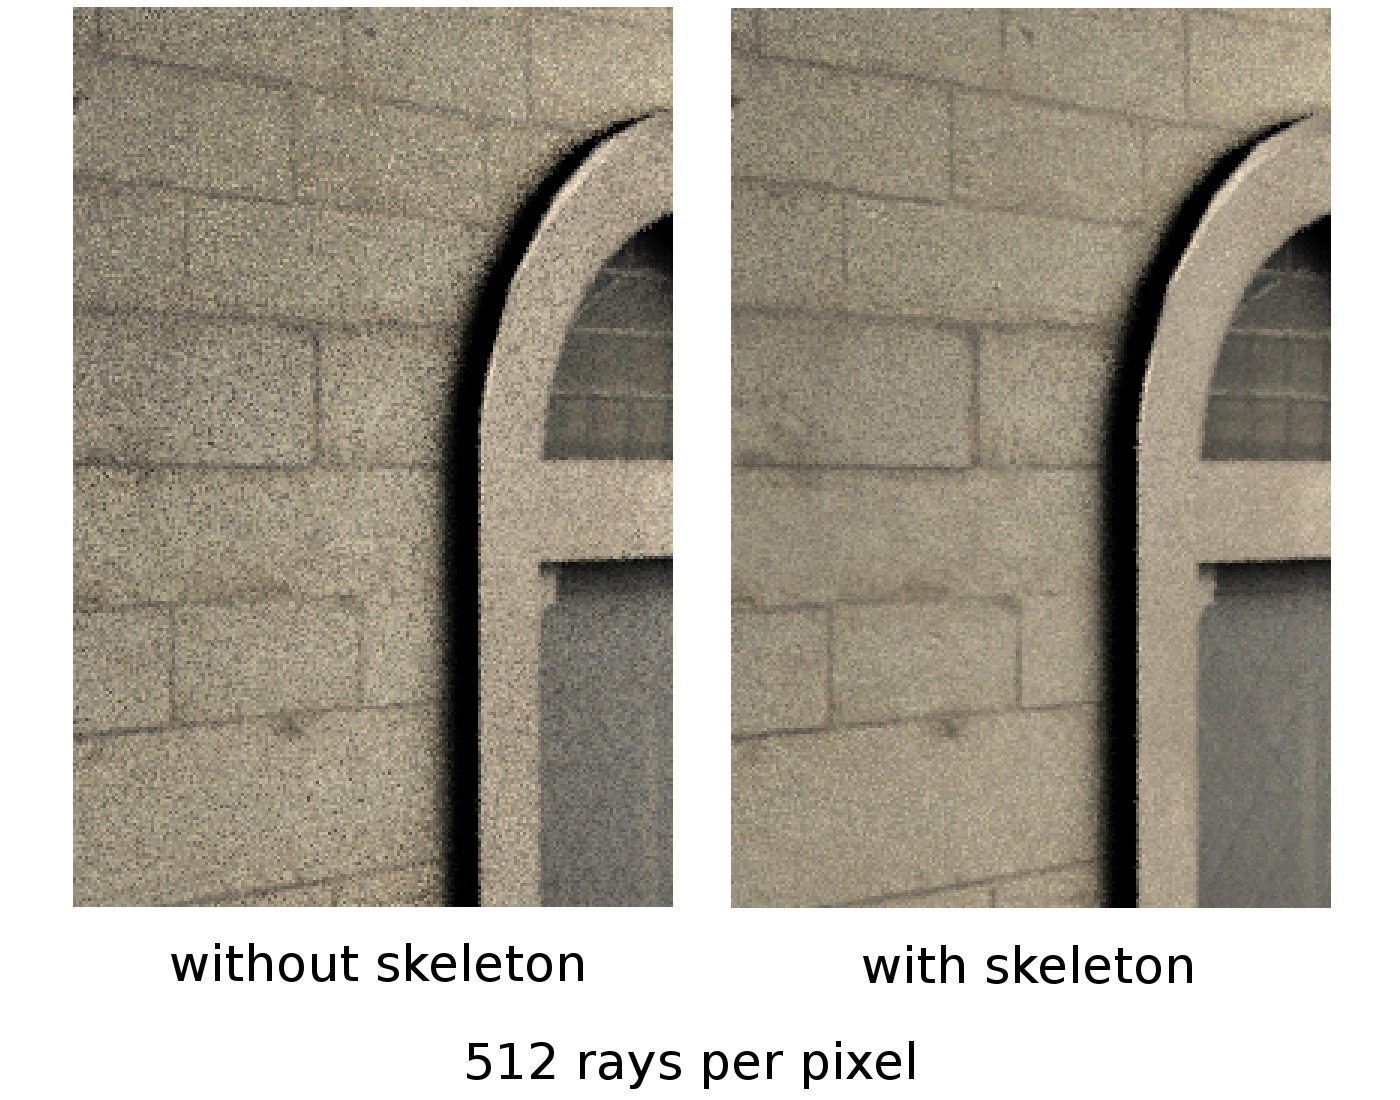
\includegraphics[scale=0.2]{images/skel_based_rt.png}
\end{center}

We observe a net decreasing of the noise: we get a faster convergence to the true image.

\subsection{Discussion}

We presented an application of our skeletonization algorithm for global illumination. Our strategy work wells, especially in dark areas. It reduces noise by taking into account the distribution of energy in the scene. One of the problem is that we take into account only one importance direction for sampling, we totally ignore the BRDF and the cosine factor. A solution called Multiple Importance Sampling allow us to combine different strategies into one. We will not describe this strategy because it's not directly related to skeletonization, but it have allowed us to improve our results and remove some artifact of our method.
